\section{数据集与切分细节}
\label{app:data}

\subsection{ScienceWorld 任务类型}

表~\ref{tab:sw_tasks}列出用于训练和分布外评测的 ScienceWorld 任务类型。

\begin{table}[h]
\centering
\small
\resizebox{\linewidth}{!}{%
\begin{tabular}{ll}
\toprule
\textbf{切分} & \textbf{任务类型} \\
\midrule
\multirow{4}{*}{训练（13）} & boil, melt, chemistry-mix, find-animal, \\
& find-plant, grow-plant, identify-life-stages-1, \\
& lifespan-longest-lived, inclined-plane-angle, \\
& measure-melting-point, power-component, \\
& test-conductivity, mendelian-genetics \\
\midrule
\multirow{4}{*}{OOD 测试（12）} & freeze, change-state-of-matter, \\
& chemistry-mix-paint, find-non-living, \\
& grow-fruit, identify-life-stages-2, \\
& lifespan-shortest, inclined-plane-friction, \\
& use-thermometer, power-renewable, \\
& test-conductivity-unknown, genetics-unknown \\
\bottomrule
\end{tabular}
}
\caption{ScienceWorld 任务类型切分。}
\label{tab:sw_tasks}
\end{table}


对于每个任务类型，我们最多采样 30 个变体（以限制收集时间）。使用固定随机种子（42）将变体按 60\%/20\%/20\% 切分为训练/验证/测试。

\subsection{HLE 学科类别}

\begin{table}[h]
\centering
\small
\begin{tabular}{lc}
\toprule
\textbf{类别} & \textbf{N（测试）} \\
\midrule
\multicolumn{2}{c}{\textit{分布内（训练）}} \\
\midrule
数学 & 200 \\
物理 & 46 \\
化学 & 23 \\
生物/医学 & 37 \\
工程 & 16 \\
计算机科学/AI & 37 \\
\midrule
\multicolumn{2}{c}{\textit{分布外}} \\
\midrule
人文/社会科学 & 193 \\
其他 & 176 \\
\bottomrule
\end{tabular}
\caption{按类别划分的 HLE 测试集分布。}
\label{tab:hle_categories}
\end{table}


\section{错误检测规则}
\label{app:error_rules}

表~\ref{tab:error_rules_detail}给出训练期间用于计算退火错误成本（AEC）的错误检测规则完整规范。每条规则包含与环境观察匹配的模式字符串、严重程度（高/中/低）和描述。

\paragraph{设计原则。}
对于 HLE，我们区分模型错误（格式违规、Python 异常）和外部失败（HTTP 错误、付费墙）。模型错误因反映可控制的失误而具有更高严重程度；外部失败依赖第三方服务，标为低严重程度。对于 ScienceWorld，我们只惩罚真正无效的动作（环境解析器无法识别的命令）。“the door is not open”或“the object is already in your inventory”之类的环境反馈属于正常探索，不被视为错误。

\paragraph{严重程度系数。}
在 AEC 中，严重程度映射到惩罚系数：高（1.0）、中（0.8）、低（0.2）。warmup 日程使用 $p_0{=}0.3$、$p_1{=}0.7$、$w_{\min}{=}0.3$ 和 $w_{\max}{=}1.0$。这些系数调节基础惩罚 $1/N$，其中 $N$ 是该任务类别的预期 episode 长度。

\begin{table*}[!htbp]
\centering
\small
\begin{tabular}{lllp{6.4cm}}
\toprule
\textbf{类别} & \textbf{规则名} & \textbf{严重程度} & \textbf{描述} \\
\midrule
\multicolumn{4}{l}{\textit{\textbf{HLE 基准}}} \\
\midrule
\multirow{4}{*}{格式错误}
 & format\_error & 中 & 工具调用格式错误---模型未遵循要求格式 \\
 & tool\_invalid\_args & 中 & 无效工具参数或缺少必需参数 \\
 & tool\_parse\_error & 中 & 工具调用解析失败 \\
 & tool\_unknown & 高 & 模型调用了不存在的工具名 \\
\midrule
\multirow{11}{*}{\shortstack[l]{Python\\执行\\错误}}
 & python\_traceback & 高 & 带 traceback 的 Python 执行异常 \\
 & python\_name\_error & 高 & 引用了未定义变量 \\
 & python\_syntax\_error & 高 & Python 语法错误 \\
 & python\_indentation\_error & 高 & Python 缩进错误 \\
 & python\_type\_error & 高 & 类型不匹配错误 \\
 & python\_value\_error & 中 & 无效值错误 \\
 & python\_index\_error & 中 & 索引越界 \\
 & python\_key\_error & 中 & 未找到字典键 \\
 & python\_attribute\_error & 中 & 属性访问错误 \\
 & python\_import\_error & 中 & 模块导入失败 \\
 & python\_zero\_division & 中 & 除零 \\
 & python\_timeout & 高 & 代码执行超时 \\
\midrule
\multirow{3}{*}{\shortstack[l]{搜索工具\\错误}}
 & search\_no\_results & 高 & 搜索未返回结果 \\
 & search\_http\_error & 低 & 搜索期间 HTTP 连接错误 \\
 & search\_rate\_limit & 低 & 超出搜索速率限制 \\
\midrule
\multirow{5}{*}{\shortstack[l]{浏览工具\\错误}}
 & browse\_403 & 低 & HTTP 403 禁止访问 \\
 & browse\_404 & 低 & HTTP 404 未找到 \\
 & browse\_access\_denied & 低 & 资源访问被拒绝 \\
 & browse\_paywall & 低 & 付费墙或订阅拦截 \\
 & browse\_timeout & 低 & 浏览请求超时 \\
\midrule
\multicolumn{4}{l}{\textit{\textbf{ScienceWorld 基准}}} \\
\midrule
无效动作 & no\_known\_action & 高 & 环境解析器无法识别的无效动作命令 \\
\bottomrule
\end{tabular}
\caption{用于退火错误成本（AEC）计算的详细错误检测规则。严重程度决定惩罚系数：高（1.0）、中（0.8）、低（0.2）。浏览工具错误标为低严重程度，因为它们反映外部失败而非模型错误。}
\label{tab:error_rules_detail}
\end{table*}


\section{额外实验}
\label{app:more_experiments}

\begin{table}[!htbp]
\centering
\small
\setlength{\tabcolsep}{5pt}
\begin{tabular}{lccc}
\toprule
基准 & 预算 & 得分/准确率$\uparrow$ & 总成本（\$）$\downarrow$ \\
\midrule
ScienceWorld & $0.5\times B$ & 45.2$\pm$3.8 & 3.6 \\
ScienceWorld & $1.0\times B$ & 53.8$\pm$3.2 & 5.7 \\
ScienceWorld & $2.0\times B$ & 55.6$\pm$3.1 & 8.1 \\
\midrule
HLE & $0.5\times B$ & 20.6$\pm$2.8 & 23.4 \\
HLE & $1.0\times B$ & 26.0$\pm$2.3 & 35.0 \\
HLE & $2.0\times B$ & 27.3$\pm$2.2 & 44.8 \\
\bottomrule
\end{tabular}
\caption{预算敏感性。放宽预算会提升性能，但存在明显的边际收益递减。}
\label{tab:budget_sweep}
\end{table}

\begin{table}[!htbp]
\centering
\scriptsize
\setlength{\tabcolsep}{3.5pt}
\resizebox{\linewidth}{!}{
\begin{tabular}{lcccccccc}
\toprule
& \multicolumn{2}{c}{ScienceWorld 测试} & \multicolumn{2}{c}{ScienceWorld OOD} & \multicolumn{2}{c}{HLE 测试} & \multicolumn{2}{c}{HLE OOD} \\
\cmidrule(lr){2-3}\cmidrule(lr){4-5}\cmidrule(lr){6-7}\cmidrule(lr){8-9}
池 & 得分$\uparrow$ & 成本$\downarrow$ & 得分$\uparrow$ & 成本$\downarrow$ & 准确率$\uparrow$ & 成本$\downarrow$ & 准确率$\uparrow$ & 成本$\downarrow$ \\
\midrule
2 模型 & 50.6$\pm$3.6 & 8.9 & 7.2$\pm$4.3 & 28.5 & 25.4$\pm$2.5 & 45.2 & 36.4$\pm$3.1 & 43.5 \\
6 模型 & 53.8$\pm$3.2 & 5.7 & 9.9$\pm$3.9 & 16.3 & 26.0$\pm$2.3 & 35.0 & 38.6$\pm$3.0 & 31.2 \\
8 模型 & 54.1$\pm$3.3 & 5.3 & 10.3$\pm$4.1 & 16.8 & 25.8$\pm$2.4 & 34.2 & 39.1$\pm$2.9 & 29.5 \\
\bottomrule
\end{tabular}}
\caption{在 2、6、8 模型设置下的候选池敏感性。}
\label{tab:pool_size}
\end{table}

\begin{table}[!htbp]
\centering
\small
\setlength{\tabcolsep}{6pt}
\begin{tabular}{lcc}
\toprule
历史预算 & ScienceWorld$\uparrow$ & HLE$\uparrow$ \\
\midrule
\texttt{max\_tokens}=2048  & 49.3$\pm$3.7 & 23.8$\pm$2.6 \\
\texttt{max\_tokens}=4096  & 52.1$\pm$3.4 & 25.3$\pm$2.4 \\
\texttt{max\_tokens}=8192  & 53.8$\pm$3.2 & 26.0$\pm$2.3 \\
\texttt{max\_tokens}=16384 & 53.5$\pm$3.3 & 26.2$\pm$2.3 \\
\bottomrule
\end{tabular}
\caption{对历史 token 预算的敏感性。}
\label{tab:history_budget}
\end{table}

\section{OpenRouter 基线细节}
\label{app:openrouter}

\paragraph{动机。}
OpenRouter~\citep{openrouter}提供自动路由 API，常用于商用部署。我们将 OpenRouter 作为代表性商用路由基线纳入，以将 \method 与现成的生产路由系统置于同一语境。

\paragraph{模型池。}
不同于将路由限制在固定 6 模型候选池（表~\ref{tab:model_pool}）的设置，OpenRouter 的自动路由可从更广泛的模型集合中选择。在我们的评测中，OpenRouter 基线在下列池中路由（由 API 在路由时报告）：

\begin{table*}[t]
\centering
\footnotesize
\begin{tabular}{ll}
\toprule
\textbf{提供商/模型} & \textbf{提供商/模型} \\
\midrule
\texttt{openai/gpt-5.1} & \texttt{openai/gpt-5} \\
\texttt{openai/gpt-5-mini} & \texttt{openai/gpt-5-nano} \\
\texttt{openai/gpt-4.1} & \texttt{openai/gpt-4.1-mini} \\
\texttt{openai/gpt-4.1-nano} & \texttt{openai/gpt-4o} \\
\texttt{openai/gpt-4o-2024-05-13} & \texttt{openai/gpt-4o-2024-08-06} \\
\texttt{openai/gpt-4o-2024-11-20} & \texttt{openai/gpt-4o-mini} \\
\texttt{openai/gpt-4o-mini-2024-07-18} & \texttt{openai/gpt-4-turbo} \\
\texttt{openai/gpt-4-turbo-preview} & \texttt{openai/gpt-4-1106-preview} \\
\texttt{openai/gpt-4} & \texttt{openai/gpt-3.5-turbo} \\
\texttt{openai/gpt-oss-120b} & \texttt{anthropic/claude-opus-4.5} \\
\texttt{anthropic/claude-opus-4.1} & \texttt{anthropic/claude-opus-4} \\
\texttt{anthropic/claude-sonnet-4.5} & \texttt{anthropic/claude-sonnet-4} \\
\texttt{anthropic/claude-3.7-sonnet} & \texttt{anthropic/claude-haiku-4.5} \\
\texttt{anthropic/claude-3.5-haiku} & \texttt{anthropic/claude-3-haiku} \\
\texttt{google/gemini-3-pro-preview} & \texttt{google/gemini-2.5-pro} \\
\texttt{google/gemini-2.0-flash-001} & \texttt{google/gemini-2.5-flash} \\
\texttt{mistralai/mistral-large} & \texttt{mistralai/mistral-large-2407} \\
\texttt{mistralai/mistral-large-2411} & \texttt{mistralai/mistral-medium-3.1} \\
\texttt{mistralai/mistral-nemo} & \texttt{mistralai/mistral-7b-instruct} \\
\texttt{mistralai/mixtral-8x7b-instruct} & \texttt{mistralai/mixtral-8x22b-instruct} \\
\texttt{mistralai/codestral-2508} & \texttt{x-ai/grok-4} \\
\texttt{x-ai/grok-3} & \texttt{x-ai/grok-3-mini} \\
\texttt{deepseek/deepseek-r1} & \texttt{meta-llama/llama-3.3-70b-instruct} \\
\texttt{meta-llama/llama-3.1-405b-instruct} & \texttt{meta-llama/llama-3.1-70b-instruct} \\
\texttt{meta-llama/llama-3.1-8b-instruct} & \texttt{meta-llama/llama-3-70b-instruct} \\
\texttt{meta-llama/llama-3-8b-instruct} & \texttt{qwen/qwen3-235b-a22b} \\
\texttt{qwen/qwen3-32b} & \texttt{qwen/qwen3-14b} \\
\texttt{cohere/command-r-plus-08-2024} & \texttt{cohere/command-r-08-2024} \\
\texttt{moonshotai/kimi-k2-thinking} & \texttt{perplexity/sonar} \\
\bottomrule
\end{tabular}
\caption{我们的 OpenRouter 基线使用的 OpenRouter 自动路由模型池（由 API 在路由时报告）。}
\label{tab:openrouter_pool}
\end{table*}


\paragraph{比较含义。}
由于 OpenRouter 可从模型超集（包括未在我们模型池中出现的多个前沿及提供商特定模型）中选择，它代表比我们的设置更强的路由场景。我们仍将其作为实用参考点纳入，但解释比较时应注意候选模型池不一致。

\paragraph{为何 OpenRouter 在 ScienceWorld 上表现较差？}
图~\ref{fig:openrouter_model_usage}展示 OpenRouter 在两个基准上的模型使用分布。在 ScienceWorld 上，OpenRouter 主要选择轻量模型：Mistral-Nemo 占全部模型调用的 68\%，其次是 GPT-5-nano（24\%）和 Claude-4.5（7\%）。这些模型虽然成本高效，却缺乏 ScienceWorld 的程序化科学任务所需的推理能力。相比之下，在 HLE 上，OpenRouter 将 54\% 的调用分配给更强的前沿模型 Claude-4.5，同时分配给 Sonar（23\%）和 Mistral-Nemo（15\%），反映了对该基准更恰当的难度评估。

这一差异揭示了通用商用路由器的一个关键局限：若没有任务特定训练，它们可能低估陌生领域难度，并过度依赖更便宜的模型。ScienceWorld 的文本接口和看似简单的命令可能使路由器误将其视为简单任务，但它实际上需要多步规划和精确动作序列，较弱模型难以执行。环境评分函数给出的负分（测试为 $-26.4$，OOD 为 $-26.9$）表明，所选模型常无法朝任务完成取得有意义的进展。

\begin{figure}[!htbp]
\centering
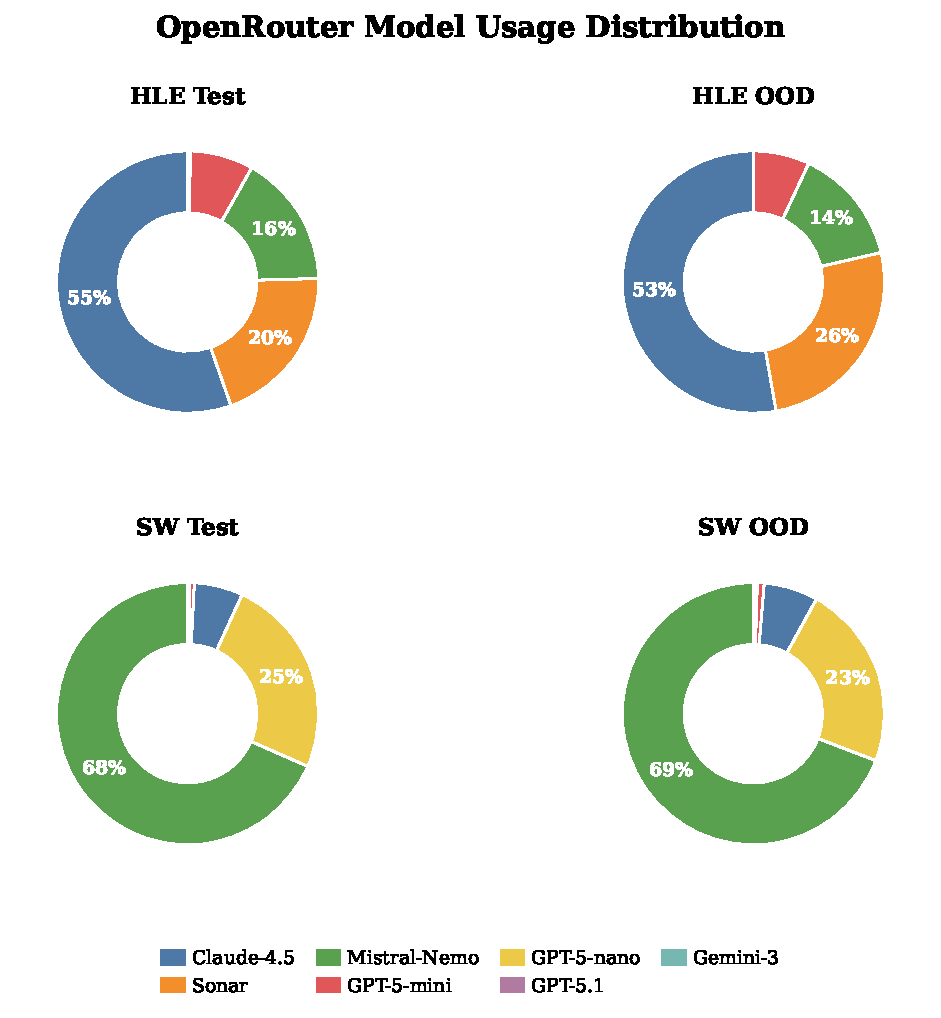
\includegraphics[width=\columnwidth]{figures/openrouter_model_usage.pdf}
\caption{OpenRouter 在 ScienceWorld 和 HLE 上的模型使用分布。在 ScienceWorld 上，OpenRouter 主要使用轻量模型（Mistral-Nemo：68\%，GPT-5-nano：24\%）；在 HLE 上，它主要使用更强模型（Claude-4.5：54\%），反映出不同的难度评估。}
\label{fig:openrouter_model_usage}
\end{figure}

\section{提示词与工具 schema}
\label{app:prompts}

我们报告评测设置中使用的提示词。为节省篇幅，省略格式错误纠正提示词。

\subsection{ScienceWorld 智能体提示词}
\label{app:prompts:sw}
\begin{figure*}[!htbp]
\begin{paperbox}{ScienceWorld 系统提示词}
你是一名与文本式科学模拟环境交互的有帮助助手。你的目标是通过发出文本命令完成科学实验。

\vspace{0.3cm}
\textbf{交互方式} \\
请将命令写在 \texttt{```text} 代码块中。环境将以观察结果回应。

\vspace{0.2cm}
\texttt{<format\_example>} \\
\texttt{THOUGHT: 我应该先探索周围环境。} \\
\texttt{```text} \\
\texttt{look around} \\
\texttt{```} \\
\texttt{</format\_example>}

\vspace{0.3cm}
\textbf{可用命令类型} \\
常见命令包括：
\begin{itemize}
\item 移动：\texttt{go to [location]}、\texttt{open door}、\texttt{go through door}
\item 交互：\texttt{pick up [object]}、\texttt{put [object] in [container]}、\texttt{activate [object]}
\item 观察：\texttt{look around}、\texttt{look at [object]}、\texttt{inventory}
\item 任务特定：\texttt{focus on [object]}、\texttt{use [tool] on [object]}
\end{itemize}

\vspace{0.2cm}
\textbf{查询命令（免费动作）} \\
你可在不消耗游戏轮次的情况下查询可用动作：
\begin{itemize}
\item \texttt{?navigation}：显示移动动作（go、walk、move）
\item \texttt{?object}：显示对象操作（pick up、put、pour）
\item \texttt{?observation}：显示观察动作（look、examine、inventory）
\item \texttt{?device}：显示设备控制（activate、turn on/off、use）
\item \texttt{?door}：显示门/容器动作（open、close）
\item \texttt{?electrical}：显示电气动作（connect、disconnect）
\item \texttt{?interaction}：显示交互动作（mix、eat、focus）
\item \texttt{?all}：显示所有有效动作
\item \texttt{?categories}：显示查询帮助
\end{itemize}
在决定下一步之前，使用查询探索可用动作。

\vspace{0.2cm}
\textbf{重要说明}
\begin{itemize}
\item 每次响应只发出\textbf{一条}命令
\item 包含解释推理的 THOUGHT 部分
\item 环境按轮次交互---在发出下一条命令前等待观察结果
\item 部分任务需要多步才能完成
\end{itemize}
\end{paperbox}
\end{figure*}

\begin{figure*}[!htbp]
\begin{paperbox}{ScienceWorld 实例提示词}
\texttt{<task\_description>} \\
\texttt{\{\{task\_description\}\}} \\
\texttt{</task\_description>}

\vspace{0.2cm}
\texttt{<initial\_observation>} \\
\texttt{\{\{initial\_observation\}\}} \\
\texttt{</initial\_observation>}

\vspace{0.2cm}
\texttt{<instructions>} \\
完成上文描述的科学实验。你正在与模拟环境交互。请一次发出一条命令并观察结果。

\vspace{0.2cm}
\textbf{提示}：使用 \texttt{?navigation} 或 \texttt{?object} 等查询命令探索可用动作，且不消耗轮次。

\vspace{0.2cm}
\textbf{策略提示：}
\begin{itemize}
\item 先探索：使用 \texttt{open door to [room]}，再使用 \texttt{go to [room]} 导航
\item 观察每个房间，寻找所需对象
\item 使用 \texttt{pick up [object]} 拾取对象
\item 加热时：找到炉灶，用 \texttt{activate [stove]} 打开，将容器放到其上
\item 冷却时：使用冷冻柜或冰箱
\item 使用 \texttt{focus on [object]} 检查物质
\end{itemize}

\vspace{0.2cm}
为完成任务，请执行任务描述所需的动作。当你认为任务完成时，发出命令：

\vspace{0.2cm}
\texttt{```text} \\
\texttt{task completed} \\
\texttt{```} \\

\vspace{0.2cm}
\textbf{请记住：}
\begin{itemize}
\item 逐步思考需要哪些动作
\item 探索环境以找到所需对象
\item 有些动作可能需要前提条件（例如先拾取对象才能使用它）
\end{itemize}
\texttt{</instructions>}
\end{paperbox}
\end{figure*}


\subsection{HLE 智能体提示词}
\label{app:prompts:hle}
HLE 系统提示词通过模板变量注入工具 schema。我们在附录~\ref{app:tool_schemas}中逐一列出每个工具 schema。
\begin{figure*}[!htbp]
\begin{paperbox}{HLE 系统提示词}
\small
你是一名专家问题求解者，正在解决 Humanity's Last Exam 中的挑战性问题。这些问题需要深入推理、谨慎研究和精确答案。

\vspace{0.15cm}
\textbf{可用工具} \\
\texttt{<tools>} \\
\texttt{\{\% for tool in tool\_schemas \%\}} \\
\texttt{\{\{ tool.to\_xml() \}\}} \\
\texttt{\{\% endfor \%\}} \\
\texttt{</tools>}

\vspace{0.15cm}
\textbf{工具调用格式} \\
你可以在 \texttt{<tool\_call>} 标签中使用 XML 或 JSON 格式：

\vspace{0.1cm}
\textbf{格式 A：XML} \\
\texttt{<tool\_call>} \\
\texttt{<tool\_name>} \\
\texttt{\ \ <param1>value1</param1>} \\
\texttt{\ \ <param2>value2</param2>} \\
\texttt{</tool\_name>} \\
\texttt{</tool\_call>}

\vspace{0.1cm}
\textbf{格式 B：JSON} \\
\texttt{<tool\_call>\{"name": "tool\_name", "arguments": \{"param1": "value1"\}\}</tool\_call>}

\vspace{0.15cm}
\textbf{示例}

\vspace{0.05cm}
\texttt{<tool\_call>} \\
\texttt{<search>} \\
\texttt{\ \ <query>maximum likelihood estimation</query>} \\
\texttt{</search>} \\
\texttt{</tool\_call>}

\vspace{0.05cm}
\texttt{<tool\_call>\{"name": "python", "arguments": \{"code": "print(2 + 2)"\}\}</tool\_call>}

\vspace{0.15cm}
\textbf{HLE 问题策略}
\begin{enumerate}[leftmargin=*, label=\arabic*., noitemsep, topsep=0pt]
\item \textbf{理解问题}：仔细阅读并识别所问内容
\item \textbf{拆分问题}：必要时将其分解为子问题
\item \textbf{必要时研究}：对不确定的事实信息使用 \texttt{search}
\item \textbf{核验来源}：准确性重要时，使用 \texttt{browse} 阅读一手来源
\item \textbf{必要时计算}：使用 \texttt{python} 进行计算和数据分析
\item \textbf{综合}：整合多个来源的信息
\item \textbf{核验答案}：提交前再次检查
\item \textbf{提交}：使用 \texttt{answer} 提交最终答案
\end{enumerate}

\vspace{0.1cm}
\textbf{重要说明}
\begin{itemize}[noitemsep, topsep=0pt]
\item 这些是挑战性问题---请从容作答
\item 务必精确---通常要求精确答案
\item 使用工具前展示你的推理
\item 若不确定，请在答案中表达置信度
\end{itemize}
\end{paperbox}
\end{figure*}

\begin{figure*}[!htbp]
\begin{paperbox}{HLE 实例提示词}
\textbf{HLE 问题} \\
\texttt{\{\% if subject \%\}} \\
\textbf{学科}：\texttt{\{\{ subject \}\}} \\
\texttt{\{\% endif \%\}}

\vspace{0.2cm}
\texttt{\{\{ question | default(task) \}\}}

\vspace{0.2cm}
\hrule
\vspace{0.2cm}

请逐步求解。使用工具进行研究与核验。使用 \texttt{answer} 工具提交最终答案：
\texttt{<tool\_call>\{"name": "answer", "arguments": \{"answer": "your final answer"\}\}</tool\_call>}
\end{paperbox}
\end{figure*}


\subsection{工具 schema}
\label{app:tool_schemas}
我们列出 HLE 智能体使用的各工具 JSON schema（名称、描述与参数 schema）。
\input{prompts/tool_schema_search_json_zh}
\input{prompts/tool_schema_browse_json_zh}
\input{prompts/tool_schema_python_json_zh}
\input{prompts/tool_schema_answer_json_zh}

\subsection{用于 LLM Router / Router-R1 的路由模型提示词}
\label{app:prompts:routing}
我们报告 LLM Router 基线和 Router-R1 使用的轮级路由提示词。两个基线在每一轮查询路由模型来产生一个 \texttt{<select>} 决策，并使用相同的提示词模板；Router-R1 使用训练后的 \texttt{Qwen2.5-7B-Instruct} 路由模型，而 LLM Router 直接使用 \texttt{DeepSeek-V3.2}（不训练）。
\begin{figure*}[!htbp]
\begin{paperbox}{LLM Router / Router-R1 系统提示词（策略 LLM）}
你是一名模型路由助手。你的工作是为给定任务选择最佳模型。

\vspace{0.3cm}
\textbf{可用模型：} \\
\texttt{\{model\_list\}}

\vspace{0.3cm}
\textbf{说明}
\begin{enumerate}[leftmargin=*, label=\arabic*.]
\item 在 \texttt{<think>...</think>} 标签中分析任务
\item 使用 \texttt{<select>model\_name</select>} 选择最佳模型
\end{enumerate}

\vspace{0.2cm}
\textbf{示例} \\
\texttt{<think>这是一个简单的数学问题。更便宜的模型已足够。</think>} \\
\texttt{<select>deepseek/deepseek-v3.2</select>}

\vspace{0.3cm}
\textbf{规则}
\begin{itemize}
\item 你必须且只能输出一个 \texttt{<select>} 标签
\item 模型名称必须与可用列表完全一致
\item 考虑任务复杂度、模型优势和成本效益
\end{itemize}
\end{paperbox}
\end{figure*}

\begin{figure*}[!htbp]
\begin{paperbox}{LLM Router / Router-R1 模型描述}
\texttt{openai/gpt-5}：成本 1.25/10，上下文 400K。SW 成功率 48\%、HLE 成功率 25\%，表现最佳。适用于复杂多步推理和困难科学问题。 \\
\texttt{openai/gpt-oss-120b}：成本 0.09/0.36，上下文 131K。SW 成功率 33\%、HLE 成功率 10\%，在中等难度任务上成本效益极佳。 \\
\texttt{moonshotai/kimi-k2-0905}：成本 0.39/1.9，上下文 131K。SW 成功率 31\%、HLE 成功率 11\%。适合通用任务，指令遵循良好。 \\
\texttt{deepseek/deepseek-v3.2}：成本 0.27/0.42，上下文 164K。SW 成功率 16\%、HLE 成功率 16\%。擅长数学和编码，适用于结构化推理任务。 \\
\texttt{google/gemini-2.5-flash-lite}：成本 0.1/0.4，上下文 1M。SW 成功率 23\%、HLE 成功率 6\%。上下文窗口最大，适用于长文档分析。 \\
\texttt{minimax/minimax-m2}：成本 0.2/1，上下文 196K。SW 成功率 22\%、HLE 成功率 8\%。推理快速，适用于简单问答和直接任务。
\end{paperbox}
\end{figure*}


\subsection{浏览提取器提示词}
\label{app:prompts:browse}
HLE 的 \texttt{browse} 工具可选择使用 LLM，从检索到的网页中提取和摘要相关证据。我们报告该基于 LLM 摘要的提取器提示词。
\begin{figure*}[!htbp]
\begin{paperbox}{浏览提取器提示词（LLM 摘要）}
请处理以下网页内容和用户目标，以提取相关信息：

\vspace{0.3cm}
\textbf{\large 网页内容} \\
\{webpage\_content\}

\vspace{0.3cm}
\textbf{\large 用户目标} \\
\{goal\}

\vspace{0.3cm}
\textbf{\large 任务指南}
\begin{enumerate}[leftmargin=*, label=\arabic*.]
\item \textbf{为推理扫描内容}：在网页内容中定位与用户目标直接相关的\textbf{具体章节/数据}。
\item \textbf{为证据提取关键信息}：从内容中识别并提取\textbf{最相关的信息}；不要遗漏重要信息。尽可能输出\textbf{完整的原始上下文}（可超过三段）。
\item \textbf{为摘要组织输出}：组织为逻辑流畅的简洁段落，优先保证清晰度，并判断信息对目标的贡献。
\end{enumerate}

\vspace{0.2cm}
\textbf{输出格式}：包含 \texttt{"rational"}、\texttt{"evidence"} 和 \texttt{"summary"} 字段的 JSON 格式。
\end{paperbox}
\end{figure*}


\subsection{HLE 裁判提示词}
\label{app:prompts:judge}
HLE 评分使用与官方 HLE 评测对齐的 LLM-as-a-judge 组件。我们报告用于将模型响应与给定参考答案比较的裁判提示词。
\begin{figure*}[!htbp]
\begin{paperbox}{HLE 裁判提示词}
根据下方精确且无歧义的 \texttt{[correct\_answer]}，判断以下对 \texttt{[question]} 的 \texttt{[response]} 是否正确。

\vspace{0.3cm}
\texttt{[question]: \{question\}} \\
\texttt{[response]: \{response\}}

\vspace{0.3cm}
你的判定必须符合以下格式和标准：

\vspace{0.2cm}
\textbf{extracted\_final\_answer}：从 \texttt{[response]} 提取的最终精确答案。若响应中没有可提取的精确最终答案，将提取结果设为 \texttt{None}。

\vspace{0.2cm}
\texttt{[correct\_answer]: \{correct\_answer\}}

\vspace{0.2cm}
\textbf{reasoning}：根据 \texttt{[correct\_answer]} 解释 extracted\_final\_answer 为何正确或错误，只关注是否存在实质性差异。不要评论背景，不要尝试解决问题，不要为不同于 \texttt{[correct\_answer]} 的答案辩护；只关注答案是否匹配。

\vspace{0.2cm}
\textbf{correct}：若 extracted\_final\_answer 与上方给定的 \texttt{[correct\_answer]} 匹配，或数值问题的误差在小范围内，回答 \texttt{yes}；否则回答 \texttt{no}。

\vspace{0.2cm}
\textbf{confidence}：从 \texttt{[response]} 提取的 0\% 到 100\% 置信度分数。若没有置信度分数可用，填 100。

\vspace{0.2cm}
以包含四个字段的 JSON 对象作答：extracted\_final\_answer、reasoning、correct、confidence。
\end{paperbox}
\end{figure*}

